% +------------------------------------------------------------------------+
% | Reference manual page: SHalfedge.tex
% +------------------------------------------------------------------------+
% | 14.05.2004   Peter Hachenberger
% | Package: Nef_3
% | 
\RCSdef{\RCSSHalfedgeRev}{$Id$}
\RCSdefDate{\RCSSHalfedgeDate}{$Date$}
% +------------------------------------------------------------------------+

\ccRefPageBegin

%%RefPage: end of header, begin of main body
% +------------------------------------------------------------------------+


\begin{ccRefClass}[Nef_polyhedron_3<Traits>::]{SHalfedge}

\ccDefinition

A shalfedge is a great arc on a sphere map. 
Figure~\ref{figureNef3HalfedgeIncidences}
depicts the relationship between a shalfedge and its incident
shalfedges, svertices, and sfaces on a sphere map.  A shalfedge is 
an oriented sedge between two svertices. It is always paired with a 
shalfedge pointing in
the opposite direction. The \ccc{twin()} member function returns
this shalfedge of opposite orientation.

    \begin{figure}[bht]
\begin{ccTexOnly}
        \begin{center}
          \parbox{0.4\textwidth}{%
              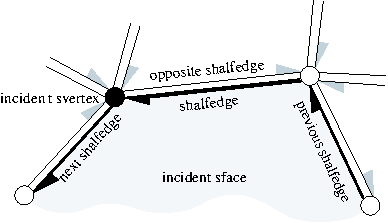
\includegraphics[width=0.4\textwidth]{Nef_3_ref/fig/shalfedge}%
          }
        \end{center}
\end{ccTexOnly}

\begin{ccHtmlOnly}
    <CENTER>
    <A HREF="fig/shalfedge.gif">
        <img src="fig/shalfedge.gif" 
             alt="Incidences of an SHalfedge"></A><BR>
    </CENTER>
\end{ccHtmlOnly}
        \label{figureNef3HalfedgeIncidences}
    \end{figure}

The \ccc{snext()} member function points 
to the successor shalfedge around this sface while the \ccc{sprev()} member 
function points to the preceding shalfedge.  An
successive assignments of the form \ccc{se = se->snext()} cycles
counterclockwise around the sface (or hole).

Similarly, the successive
assignments of the form \ccc{se = se->snext()->twin()} cycle
clockwise around the svertex and traverse all halfedges incident to
this svertex. The assignment \ccc{se = se->cyclic_adj_succ()} can be 
used as a shortcut.

The role of shalfedges in a facet is illustrated in 
Figure~\ref{figureNef3FacetIncidences}.
The \ccc{facet()} member function returns the facet in which
the shalfedge is part of one of the facet cycles. The successive assignment of 
the form \ccc{se = se->next()} cycles counterclockwise around the facet (or a
hole of the facet).

A const circulators is provided for each of the three circular orders.
The circulators are bidirectional and assignable to \ccc{SHalfedge_const_handle}.

\ccInclude{CGAL/Nef_polyhedron_3.h}

\ccTypes
\ccThree{SHalfedge_const_handle}{se.cyclic_adj_pred();;}{}
\ccThreeToTwo

The following types are the same as in \ccc{Nef_polyhedron_3<Traits>}.

\ccNestedType{Mark}{type of mark.}

\ccNestedType{Sphere_circle}{sphere circle type stored in SHalfedge.}

\ccNestedType{Halffacet_const_handle}{const handle to Halffacet.}
\ccGlue
\ccNestedType{SVertex_const_handle}{const handle to SVertex.}
\ccGlue
\ccNestedType{SHalfedge_const_handle}{const handle to SHalfedge.}
\ccGlue
\ccNestedType{SFace_const_handle}{const handle to SFace.}

\ccCreation
\ccCreationVariable{se}

There is no need for a user to create a \ccc{SHalfedge} explicitly. The
class \ccc{Nef_polyhedron_3<Traits>} manages the needed shalfedges internally.

%\ccConstructor{SHalfedge();}{default constructor.}

\ccOperations

\ccMethod{const Mark& mark() const;}{the mark of \ccVar\ .}

\ccMethod{const Sphere_circle& circle() const;}{the sphere circle of \ccVar\ .}

\ccMethod{SHalfedge_const_handle twin() const;}{the twin of \ccVar\ .}

\ccMethod{SVertex_const_handle source() const;}{the source svertex of \ccVar\ .}

\ccMethod{SVertex_const_handle target() const;}{equals \ccc{twin()->source()}.}

\ccMethod{SHalfedge_const_handle prev() const;}
{the SHalfedge previous to \ccVar\ in a facet cycle.}

\ccMethod{SHalfedge_const_handle next() const;}
{the next SHalfedge of \ccVar\ in a facet cycle.}

\ccMethod{SHalfedge_const_handle sprev() const;}
{the SHalfedge previous to \ccVar\ in a sface cycle.}

\ccMethod{SHalfedge_const_handle snext() const;}
{the next SHalfedge of \ccVar\ in a sface cycle.}

\ccMethod{SHalfedge_const_handle cyclic_adj_pred() const;}
{the edge before \ccVar\ in the cyclic ordered adjacency list of source().}

\ccMethod{SHalfedge_const_handle cyclic_adj_succ() const;}
{the edge after \ccVar\ in the cyclic ordered adjacency list of source().}

\ccMethod{Halffacet_const_handle facet() const;}
{the facet that corresponds to \ccVar\ in the 3D incidence structure.}

\ccMethod{SFace_const_handle incident_sface() const;}{the incident
  sface of \ccVar\ .}

\ccMethod{bool in_outer_sface_cycle() const; }{determines whether \ccVar\ is
  in an outer sface cycle.}

\ccMethod{bool in_inner_sface_cycle() const; }{determines whether \ccVar\ is
  in an inner sface cycle.}

\ccMethod{bool in_outer_facet_cycle() const; }{determines whether \ccVar\ is
  in an outer facet cycle.}

\ccMethod{bool in_inner_facet_cycle() const; }{determines whether \ccVar\ is
  in an inner facet cycle.}


\ccSeeAlso

\ccRefIdfierPage{CGAL::Nef_polyhedron_3<Traits>::Halfedge}\\
\ccRefIdfierPage{CGAL::Nef_polyhedron_3<Traits>::Halffacet}\\
\ccRefIdfierPage{CGAL::Nef_polyhedron_3<Traits>::SFace}\\
\ccRefIdfierPage{CGAL::Nef_polyhedron_S2<Traits>::Sphere_circle}

\ccTagDefaults
\end{ccRefClass}

% +------------------------------------------------------------------------+
%%RefPage: end of main body, begin of footer
\ccRefPageEnd
% EOF
% +------------------------------------------------------------------------+
